%%%%%%%%%%%%%%%%%%%%%%%%%%%%%%%%%%%%%%%%%%%%%%%%%%%%%%%%%%%%%%%%%
%% Section 5.3 was written before I read Section 6.1
%% these slides contain most of the material from both sections.
%%%%%%%%%%%%%%%%%%%%%%%%%%%%%%%%%%%%%%%%%%%%%%%%%%%%%%%%%%%%%%%%%

\begin{frame}{Hypothesis Testing Framework}
    Suppose we're interested in examining how people perform on a multiple choice question related to world health. We might like to understand if
    
    \vspace{12pt}$\boldsymbol{H_0}$: People never learn these topics and their responses are random guesses.
    
    \vspace{12pt}$\boldsymbol{H_A}$: People have knowledge that helps them do better than random guessing, or perhaps have false knowledge that leads them to do worse than random guessing.
\end{frame}

\begin{frame}{Hypotheses}
    We talked briefly about hypothesis before! Recall that
    \begin{itemize}
        \item $H_0$ is the \textbf{null hypothesis}.
        \item $H_A$ is the \textbf{alternative hypothesis}.
    \end{itemize}
\end{frame}

\begin{frame}{Hypotheses}
    \begin{itemize}
        \item The null hypothesis represents a skeptical perspective or a perspective of "no difference". This is the claim to be tested.
        \item The alternative hypothesis is some new, alternate claim. It is often represented by a range of possible values.
    \end{itemize}
    We will define these more precisely as we go.
\end{frame}

\begin{frame}{Hypotheses}
    Let's return to our example about a world health question.  
    \begin{itemize}
        \item Suppose there are 4 possible answers and only 1 correct answer.
        \item The responses being random guesses corresponds to
        \[
            H_0: p = \frac{1}{4}
        \]
        \item The responses relating to some knowledge (whether correct or incorrect) corresponds to
        \[
            H_A: p \ne \frac{1}{4}
        \]
    \end{itemize}
\end{frame}

\begin{frame}{Hypotheses}
    The alternative hypothesis usually represents a new or stronger perspective.
    \begin{itemize}
        \item It would be interesting to know that people know something about world health (if in fact $p>1/4$).
        \item It would also be interesting to know if people have misleading information about world health (if in fact $p<1/4$).
    \end{itemize}
\end{frame}

\begin{frame}{Hypothesis Testing}
    The hypothesis testing framework is very general!
    \begin{itemize}
        \item Any time someone makes a claim that's difficult to believe, we start by being skeptical.
        \item If enough evidence is presented to support that claim, we may reject our skeptical position and change our minds.
    \end{itemize}
\end{frame}

\begin{frame}{Example: Juries}
    A jury on a criminal case makes two possible decisions: innocent or guilty.
    
   \vspace{12pt}In principle, the US court system operates under "innocent until proven guilty".  
    
    \vspace{12pt}How might we set this up in a formal hypothesis framework?
\end{frame}

\begin{frame}{Example: Juries}
    If a person is innocent until proven guilty, our default assumption should be that the person is innocent:
    \[
        \boldsymbol{H_0}: \text{ the defendant is innocent. }
    \]
    We should be skeptical of the claim that a person is guilty, concluding guilt only if we are convinced beyond a reasonable doubt:
    \[
        \boldsymbol{H_A}: \text{ the defendant is guilty. }
    \]
\end{frame}

\begin{frame}{Example: Juries}
    \begin{itemize}
        \item Crucially, even if we aren't convinced that a person is innocent, we may still fail to convict.
        \item That is, we may fail to convict because we are unsure.
        \item This is because a jury's decision is based on our being overwhelmingly convinced of \textit{guilt}, not of innocence.
        \item The prosecutor may fail to provide enough evidence to convince us of guilt, but that doesn't necessarily mean that the defendant is innocent. 
    \end{itemize}
\end{frame}

\begin{frame}{Hypothesis Testing}
    The jury framework is a lot like hypothesis testing:
    \begin{itemize}
        \item We may find sufficient evidence to reject the null hypothesis.
        \item We may also not find sufficient evidence to reject the null hypothesis.
        \item However, even if we lack this evidence, we typically do not accept the null hypothesis as true. 
        \item Failing to find sufficient evidence for the alternative hypothesis does not necessarily mean that the null hypothesis is true!
    \end{itemize}
\end{frame}

\begin{frame}{Hypotheses}
    Let's return to our example about a world health question.  
    \begin{itemize}
        \item Recall that
        \[
            H_0: p = \frac{1}{4}
        \]
        \item and
        \[
            H_A: p \ne \frac{1}{4}.
        \]
    \end{itemize}
\end{frame}

\begin{frame}{The Null Value}
    \begin{itemize}
        \item In this setting, we want to know something about the population parameter $p$. 
        \item We compare this to the value $0.25$, called the \textbf{null value}.
        \item We denote the null value by $p_0$ ("p-nought"). Here, $p_0=0.25$.
    \end{itemize}
\end{frame}

\begin{frame}{Example}
    \begin{itemize}
        \item It may seem impossible that the proportion of people who get the right answer is \textit{exactly} chance level ($p=0.25$).
        \item However, recall that our framework requires that there be strong evidence in order to reject this notion.
        \item We are not trying to conclude that $p=0.25$ (we don't tend to conclude the null hypothesis).
        \item If the proportion is $0.2501$ rather than exactly $0.25$, we haven't really learned anything interesting.
    \end{itemize}
\end{frame}

\begin{frame}{Hypothesis Testing Using Confidence Intervals}
    We will use the \texttt{Rosling responses} data set to evaluate the hypothesis test evaluating whether college-educated adults get a question about infant vaccination correct. 
    
    \vspace{12pt}The question posed is: \textit{How many of the world's 1 year old children today have been vaccinated against some disease?}
    \begin{enumerate}
        \item 20\%
        \item 50\%
        \item 80\%
    \end{enumerate}
\end{frame}

\begin{frame}{Example}
    \begin{itemize}
        \item We want to know if the proportion of college-educated adults who get the question correct is different from 33.3\%.
        \item The data set summarizes the answers of 50 college-educated adults.
        \item Of these 50 adults, 24\% of respondents got the question correct (80\% of 1 year olds have been vaccinated against some disease).
    \end{itemize}
\end{frame}

\begin{frame}{Example}
    Now that we have data, we might wonder if the data provide strong evidence that the proportion of college-educated adults is different than 33.3\%.
    \begin{itemize}
        \item We know that there is fluctuation from one sample to another.
        \item We also know that it is unlikely that $\hat{p}$ will exactly equal $p$.
        \item Still, we want to draw a conclusion about $p$.
    \end{itemize}
\end{frame}

\begin{frame}{Example}
    We need to know if our sample statistic $\hat{p}=0.24$
    \begin{itemize}
        \item suggests that the true proportion is something other than $p=0.333$ 
    \end{itemize}
    OR
    \begin{itemize}
        \item if this deviation is due to random chance.
    \end{itemize}
    
    \vspace{12pt}We know how to quantify the uncertainty in our estimate using confidence intervals. How can we apply this concept to hypothesis tests?
\end{frame}

\begin{frame}{Example}
    Construct a 95\% confidence interval for $p$ using the \texttt{Rosling responses} data.
\end{frame}

\begin{frame}{Example}
    First we need to confirm that the Central Limit Theorem applies to this data.
    \[
        n\hat{p} = 50\times0.24 = 12 \ge 10
    \]
    and 
    \[
        n(1-\hat{p}) = 50\times0.76 = 38 \ge 10
    \]
    The success-failure condition holds, so we can move on to building our interval.
\end{frame}

\begin{frame}{Example}
    \begin{itemize}
        \item The point estimate is $\hat{p}=0.24$.
        \item $\alpha = 1-0.95=0.05$
        \item The critical value is $z_{0.05/2} = z_{0.025} = 1.96$
        \item The standard error is
        \[
            SE_{\hat{p}} = \sqrt{\frac{\hat{p}(1-\hat{p})}{n}} = 0.060
        \]
    \end{itemize}
\end{frame}

\begin{frame}{Example}
    Then
    \begin{align*}
        \hat{p} &\pm z_{\alpha/2} \times SE_{\hat{p}} \\
        0.24 &\pm 1.96 \times 0.060 \\
    \end{align*}
    which is the interval $(0.122, 0.358)$.
    
    \vspace{12pt}We can be 95\% confident that the proportion of college-educated adults to correctly answer the infant vaccination question is between 12.2\% and 35.8\%. 
\end{frame}

\begin{frame}{Hypothesis Testing Using Confidence Intervals}
    So we have a confidence interval... now what?
    
    \vspace{12pt}Our interval is $(0.122, 0.358)$.
    \begin{itemize}
        \item We are interested in the null value $p_0 = 0.333$.
        \item Notice that $p_0=0.333$ falls within our interval.
        \item Therefore $p_0=0.333$ is in our range of plausible values.
    \end{itemize}
    Since $p_0=0.333$ is one of our plausible values, we cannot say that the null value is implausible.
\end{frame}

\begin{frame}{Example}
    Note that we cannot make the claim that college-educated adults simply guess on this question!
    \begin{itemize}
        \item Failing to reject $H_0$ is not the same thing as concluding $H_0$.
        \item There are still lots of other plausible values that are different from $p_0=0.333$!
        \item It is possible that there is a difference that we were unable to detect with this particular study. 
    \end{itemize}
\end{frame}

\begin{frame}{Double Negatives in Statistics}
    \begin{itemize}
        \item We use a lot of double negatives when talking about hypotheses.
        \item We might say things like
        \begin{itemize}
            \item "the null hypothesis is not implausible"
            \item "we failed to reject the null hypothesis"
        \end{itemize}
        \item We use these to say that we are not rejecting, but are also not accepting, the null. 
    \end{itemize}
\end{frame}

\begin{frame}{Hypothesis Testing Using Confidence Intervals}
    Essentially, if $p_0$ is within the interval $\hat{p} \pm MoE$, then we do not reject the null hypothesis.
    
    \vspace{12pt}If $p_0$ is \textit{not} within the interval $\hat{p} \pm MoE$, then we reject the null hypothesis and conclude the alternative.
\end{frame}

\begin{frame}{Decision Errors}
    \begin{itemize}
        \item It is entirely possible that we make the right conclusion based on our data... but the wrong conclusion based on the true (unknown) parameter!
        \item In our criminal court example, sometimes people are wrongly convicted. Other times, guilty people are not convicted at all.
        \item Unlike in the courts, statistics gives us the tools to quantify how often we make these sorts of errors.
    \end{itemize}
\end{frame}

\begin{frame}{Decision Errors}
    \begin{itemize}
        \item There are two competing hypotheses: null and alternative.
        \item In a hypothesis test, we make some statement about which might be true.
        \item There are four possible scenarios. We can
        \begin{enumerate}
            \item Reject $H_0$ when $H_0$ is false.
            \item Fail to reject $H_0$ when $H_0$ is true.
            \item Reject $H_0$ when $H_0$ is true (error).
            \item Fail to reject $H_0$ when $H_0$ is false (error).
        \end{enumerate}
    \end{itemize}
    
\end{frame}

\begin{frame}{Decision Errors}
    \begin{center}
        \begin{tabular}{llcc}
             & & \multicolumn{2}{c}{\textbf{Test Conclusion}} \\ \cline{3-4} 
             & & Do not reject $H_0$ & Reject $H_0$ \\ \cline{2-4} 
            \multirow{2}{*}{\textbf{Truth}} 
                & $H_0$ true  & Correct Decision & \textbf{Type I Error} \\     & $H_0$ false & \textbf{Type II Error} & Correct Decision \\ \cline{2-4}
        \end{tabular}
    \end{center}
    \begin{itemize}
        \item A \textbf{Type 1 Error} is rejecting $H_0$ when it is actually true.
        \item A \textbf{Type 2 Error} is failing to reject $H_0$ when the $H_A$ is actually true.
    \end{itemize}
\end{frame}

\begin{frame}{Example}
    Let's think about our criminal court example. Recall that the null hypothesis is innocence.
    
    \begin{itemize}
        \item A Type I error is when we decide that a person is guilty, even though they are innocent.
        \item A Type II error is when we decide that we do not have enough evidence to say that someone is guilty, but they are in fact guilty.
    \end{itemize}
\end{frame}

\begin{frame}{Example}
    How could we reduce the Type 1 Error rate in US criminal courts? 
    
    \vspace{12pt}To lower the Type 1 Error rate, we might raise our standard for conviction from “beyond a reasonable doubt” to “beyond a conceivable doubt” so fewer people would be wrongly convicted. 
\end{frame}

\begin{frame}{Example}
    What influence might this have on the Type 2 Error rate?

    \vspace{12pt}Raising our standard for conviction would also make it more difficult to convict the people who are actually guilty, so we would make more Type 2 Errors.
\end{frame}

\begin{frame}{Error Trade-Offs}
    \begin{itemize}
        \item In general, reducing the Type I error rate increases the Type II error rate.
        \item Similarly, reducing the Type II error rate increases the Type I error rate.
        \item We see a lot of these trade-offs in statistics.
    \end{itemize}
\end{frame}

\begin{frame}{Decision Errors}
    \begin{itemize}
        \item Hypothesis testing is built around rejecting or failing to reject the null hypothesis.
        \item But when do we have "strong enough" evidence?
        \item We usually build our tests around Type I error.
        \item If the null is actually true, we do not want to incorrectly reject any more than, say 5\% of the time.
        \item This corresponds to a significance level of $\alpha=0.05$
    \end{itemize}
\end{frame}

\begin{frame}{Significance Levels}
    We talked about significance level $\alpha$ in our discussion about confidence intervals. It comes into play again here!
    \begin{itemize}
        \item The significance level indicates how often the data will lead us to incorrectly reject $H_0$
        \item This is also how often we commit a Type I error!
        \item In fact, $\alpha$ is the probability of committing such an error
        \[
            \alpha = P(\text{Type I error})
        \]
    \end{itemize}
\end{frame}

\begin{frame}{Significance Levels}
    If we use a 95\% confidence interval for hypothesis testing and the null is true,
    \begin{itemize}
        \item The significance level is $\alpha=0.05$.
        \item We make an error whenever the point estimate is at least 1.96 standard errors away from the population parameter.
        \item This happens about 5\% of the time
    \end{itemize}
\end{frame}

\begin{frame}{Hypothesis Testing Using Confidence Intervals}
    \begin{itemize}
        \item Confidence intervals can be very useful in hypothesis testing.
        \item However, sometimes we are unable to construct a confidence interval.
        \item For example, what if we wanted to consider something like
            \[ H_0: p_1=p_2=p_3=p_4 \]
        \item Therefore we want to develop a more general hypothesis testing framework.
    \end{itemize}
\end{frame}

\begin{frame}{Formal Testing Using P-Values and Test Statistics}
    \begin{itemize}
        \item We want a way to consider the strength of the evidence against the null hypothesis and in favor of the alternative hypothesis. 
        \item Instead of using confidence intervals, we use:
        \begin{itemize}
            \item p-values.
            \item test statistics.
        \end{itemize}
    \end{itemize}
\end{frame}

\begin{frame}{P-Values}
    The \textbf{p-value} is the probability of observing data at least as favorable to the alternative hypothesis as our current data set, if the null hypothesis were true. 
    
    \vspace{12pt}We typically use a summary statistic of the data, in this section the sample proportion, to help compute the p-value and evaluate the hypotheses.
\end{frame}

\begin{frame}{Test Statistics}
    \begin{itemize}
        \item A \textbf{test statistic} is a value based on the sample data.
        \item This is the z-score for the point estimate.
        \item The test statistic can be used to find a p-value (and vice versa).
    \end{itemize}
    In a hypothesis testing framework, using the test statistic and using the p-value are equivalent. 
\end{frame}

\begin{frame}{Critical Value}
    \begin{itemize}
        \item We used critical values before when building confidence intervals:
        \[
            z_{\alpha/2}
        \]
        \item Critical values in the hypothesis testing framework are the same idea.
        \item If the null hypothesis is true, the \textbf{critical value} corresponds to the maximum amount of Type I error allowed. 
    \end{itemize}
\end{frame}

\begin{frame}{Example: Coal}
    Pew Research asked a random sample of 1000 American adults whether they supported the increased usage of coal to produce energy. Set up hypotheses to evaluate whether a majority of American adults support or oppose the increased usage of coal.
\end{frame}

\begin{frame}{Example: Coal}
    \begin{itemize}
        \item Let $p$ be the true proportion who support coal.
        \item The uninteresting result is that there is no majority either way.
        \item In this case, half would support and half would oppose ($p_0=0.5$).
        \item Alternatively, there is a majority support or oppose.
    \end{itemize}
    \begin{align*}
        H_0: &\quad p = 0.5 \\
        H_A: &\quad p \ne 0.5
    \end{align*}
\end{frame}

\begin{frame}{Hypothesis Testing}
    \begin{itemize}
        \item We want to work with the normal distribution, so we need to check our success-failure condition.
        \item Whenever we use the Central Limit Theorem, we want to use the true parameter but typically don't have it.
        \item With hypothesis testing, $p_0$ is the \textit{proposed} value for $p$.
        \item We will therefore use $p_0$ in place of $p$ in our plug in method.
    \end{itemize}
\end{frame}

\begin{frame}{Hypothesis Testing}
    We use $p_0$ in place of $p$ for good reason:
    \begin{itemize}
        \item We are interested in how unlikely our observed statistic is \textit{under the condition} that the null hypothesis is true.
        \item If the null hypothesis is true, then $p=p_0$.
    \end{itemize}
\end{frame}

\begin{frame}{Example: Coal}
    What would the sampling distribution of $\hat{p}$ look like if the null hypothesis were true?
    
    \vspace{12pt}We assume that our poll is based on a random sample, so independence is satisfied. Using $p_0$ to check our success-failure condition,
    \[
        np_0 = n(1-p_0) \overset{H_0}{=} 1000\times0.5 = 500
    \]
    So we are comfortable working with a normal distribution.
\end{frame}

\begin{frame}{Example: Coal}
    Under the null hypothesis, the normal distribution for this context has mean
    \[
        \mu \overset{H_0}{=} p_0 = 0.5
    \]
    and standard error
    \[
        SE \overset{H_0}{=} \sqrt{\frac{p_0(1-p_0)}{n}} = 0.016
    \]
    Under the null hypothesis, $\hat{p} \sim N(0.5, 0.016)$.
\end{frame}

\begin{frame}{Example: Coal}
    \begin{itemize}
        \item Pew Research’s sample suggests that 37\% of American adults support increased usage of coal. 
        \item Does 37\% represent a real difference from the null hypothesis of 50\%?
    \end{itemize}
\end{frame}

\begin{frame}{Example: Coal}
    \begin{center}
        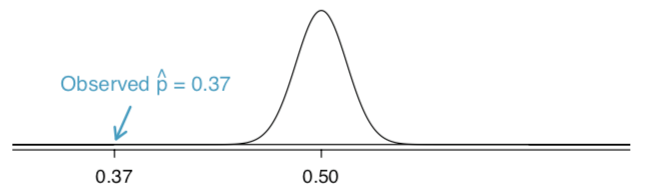
\includegraphics[scale=0.5]{images/nulldist.png}
    \end{center}
    This is the sampling distribution under the null hypothesis. We call this the \textbf{null distribution}. 
\end{frame}

\begin{frame}{Example: Coal}
    If the null hypothesis were true, determine the chance of finding $\hat{p}$ at least as far into the tails as 0.37 under the null distribution $\hat{p} \sim N(0.5, 0.016)$.
\end{frame}

\begin{frame}{Example: Coal}
    \begin{itemize}
        \item This is a normal probability problem where $x = 0.37$.
        \item First, we draw a simple graph to represent the situation.
        \item We know that $\hat{p}$ is far in the tail, so the z-score should be far from 0.
        \item Equivalently, this tail area should be quite small. 
    \end{itemize}
\end{frame}

\begin{frame}{Example: Coal}
    This Z-score is our test statistic.
    \begin{align*}
        ts = z &= \frac{\hat{p}-p_0}{SE} \\
        &= \frac{0.37 - 0.5}{0.016} \\
        &= −8.125 
    \end{align*}
    
    \vspace{12pt}The observed proportion of 0.37 is over 8 standard deviations below the mean! If the null distribution were true, there would be almost no chance of seeing such an extreme observation.
\end{frame}

\begin{frame}{Example: Coal}
    To find the p-value, we find the corresponding tail area. 
    \begin{itemize}
        \item Using software, $P(Z < -8.125) = 2.2 \times 10^{−16}$.
        \item To account for values as least as extreme in the other tail area, we double this value.
        \[
            2\times P(Z < -8.125) = 4.4 \times 10^{−16}.
        \]
    \end{itemize}
    
    \vspace{12pt}This means that there is essentially no chance that we would see a proportion of 0.34 in a sample size of 1000 if the null distribution were true!
\end{frame}

\begin{frame}{Calculating a Test Statistic}
    In general, for proportions where the Central Limit Theorem holds, the test statistic is
    \[
        ts = z = \frac{\hat{p}-p_0}{SE} =  \frac{\hat{p}-p_0}{\sqrt{\frac{p_0(1-p_0)}{n}}}
    \]
\end{frame}

\begin{frame}{Calculating a P-Value}
    Once you've calculated the test statistic, the p-value is
    \[
        2\times P(|Z| > |ts|)
    \]
\end{frame}

\begin{frame}{Hypothesis Testing Using Test Statistics}
    We compare the test statistic to the critical value to evaluate $H_0$.
    
    \vspace{12pt}When the test statistic is more extreme than the critical value, 
    \[
        |ts| > |z_{\alpha/2}|
    \]
    we reject $H_0$. Otherwise, we do not reject $H_0$.
\end{frame}

\begin{frame}{Hypothesis Testing Using P-Values}
    Equivalently, we may compare the p-value to $\alpha$ to evaluate $H_0$.
    
    \vspace{12pt}When the p-value is less than the significance level,
    \[
        \text{p-value} < \alpha
    \]
        we reject $H_0$. Otherwise, we do not reject $H_0$.
\end{frame}

\begin{frame}{Hypothesis Testing}
    If either 
    \[
        |ts| > |z_{\alpha/2}|
    \]
    or 
    \[
        \text{p-value} < \alpha
    \]
    The data provide strong evidence supporting the alternative hypothesis. 
    
    \vspace{12pt}Otherwise, we report that we do not have sufficient evidence to reject the null hypothesis. We will always describe the conclusion in the context of the data.
\end{frame}

\begin{frame}{Example}
    A simple random sample of 1028 US adults in March 2013 show that 56\% support nuclear arms reduction. Does this provide convincing evidence that a majority of Americans supported nuclear arms reduction at the 5\% significance level?
\end{frame}

\begin{frame}{Example}
    Checking our conditions for normality,
    \begin{itemize}
        \item Independence: this is a simple random sample.
        \item Success-failure: 
        \[
            np_0 = n(1-p_0) = 514 \ge 10
        \]
    \end{itemize}
    So we can model $\hat{p}$ using a normal distribution.
\end{frame}

\begin{frame}{Example}
    Now we want to calculate the standard error:
    \[
        SE = \sqrt{\frac{p_0(1-p_0)}{n}} = \sqrt{\frac{0.5\times0.5}{1028}} = 0.0156
    \] 
\end{frame}

\begin{frame}{Example: Test Statistic Approach}
    The test statistic can be computed in terms of our null model:
    \[
     ts = z = \frac{\hat{p} - p_0}{SE} = \frac{0.56 - 0.5}{0.0156} = 3.75
    \]
    The critical value for $\alpha=0.05$ is $z_{0.05/2} = 1.64$. Since
    \[
        |3.75| > |1.96|
    \]
    we can reject $H_0$ at the $\alpha=0.05$ level of significance and conclude that a majority of Americans support nuclear arms reduction. 
\end{frame}

\begin{frame}{Example: P-Value Approach}
    The p-value is the probability of being more extreme than the observed test statistic. We should draw a picture. Then using software:
    \[
        2 \times P(Z > 3.75) = 0.0002
    \]
    Since
    \[
        \text{p-value} = 0.0002 < \alpha = 0.05
    \]
    we can reject $H_0$ at the $\alpha=0.05$ level of significance and conclude that a majority of Americans support nuclear arms reduction.
\end{frame}

\begin{frame}{Hypothesis Testing for a Single Proportion}
    Once you've determined a one-proportion hypothesis test is the correct procedure, there are four steps to completing the test:
    \begin{enumerate}
        \item Identify the parameter of interest, list hypotheses, identify the significance level, and identify $\hat{p}$ and $n$.
        \item Verify that $\hat{p}$ is nearly normal under $H_0$. Use the null value in place of $p$.
        \item If the conditions hold, compute the standard error under $H_0$, compute the Z-score, and (optionally) identify the p-value.
        \item Evaluate by either comparing $ts$ to $z_{\alpha/2}$ or p-value to $\alpha$. 
    \end{enumerate}
    Make sure to provide your conclusion in the context of the problem!
\end{frame}

\begin{frame}{Choosing a Significance Level}
    \begin{itemize}
        \item The standard significance level for most fields is $\alpha=0.05$
        \item Sometimes we may adjust the significance level based on application.
        \begin{itemize}
            \item For example, if making a Type I error is especially problematic, we might reduce our significance level slightly.
            \item If making a Type II error is especially problematic, we might increase our significance level slightly.
        \end{itemize}
        \item Collecting more data also reduces Type II error, so whenever reasonable it's a good idea to collect more data!
    \end{itemize}
\end{frame}

\begin{frame}{Statistical Significance vs Practical Significance}
    \begin{itemize}
        \item For very large sample sizes, point estimates can become very precise.
        \item In these cases, differences between the point estimate and null value become easier to detect.
        \item Sometimes we can detect even an incredibly small difference!
        \item These differences are statistically significant, but may not be practically significant.
    \end{itemize}
\end{frame}

\begin{frame}{Statistical Significance vs Practical Significance}
    For example, 
    \begin{itemize}
        \item An online experiment might identify that placing additional ads on a movie review website statistically significantly increases viewership of a TV show by 0.001\%.
        \item But... who cares about an increase of 0.001\%?
        \item This increase probably has no practical value.
    \end{itemize}
\end{frame}

\begin{frame}{One-Sided Hypotheses}
    So far we've considered only \textbf{two-sided hypotheses}:
    \begin{align*}
        H_0&: \quad p = p_0 \\
        H_A&: \quad p \ne p_0
    \end{align*}
    Think of two-sided as when the alternative hypothesis has values \textit{on either side} of the null proportion. 
\end{frame}

\begin{frame}{One-Sided Hypotheses}
    For a \textbf{one-sided hypothesis test}, the alternative hypothesis has values on only one side of the null proportion. Either
    \[
        H_A: \quad p > p_0
    \]
    or
    \[
        H_A: \quad p < p_0
    \]
\end{frame}

\begin{frame}{One-Sided Hypotheses}
    We ALWAYS use equality in our null hypothesis! By convention, we write
    \begin{align*}
        H_0&: \quad p \le p_0 \\
        H_A&: \quad p > p_0
    \end{align*}
    or
    \begin{align*}
        H_0&: \quad p \ge p_0 \\
        H_A&: \quad p < p_0
    \end{align*}
\end{frame}

\begin{frame}{One-Sided Hypothesis Testing}
    There is only one major difference in one-sided hypothesis testing.
    
    \begin{itemize}
        \item For the test statistic approach
        \begin{itemize}
            \item We use the critical value $z_{\alpha}$ instead of $z_{\alpha/2}$.
        \end{itemize}
        \item For the p-value approach
        \begin{itemize}
            \item We no longer multiply by two: p-value $= P(|Z| > |ts|)$
        \end{itemize}
    \end{itemize}
\end{frame}

\begin{frame}{One-Sided Hypothesis Testing}
    In both cases,
    \begin{itemize}
        \item We are no longer interested in seeing observations as extreme as $\hat{p}$.
        \item Now we are actively interested in a particular direction corresponding to the direction of the alternative hypothesis.
        \item This means that we are interested in a particular Z-score or a single tail area.
    \end{itemize}
\end{frame}

\begin{frame}{One-Sided Hypothesis Testing}
    This is useful for several reasons
    \begin{enumerate}
        \item We don't have to find $z_{\alpha/2}$ or double the p-value, so the level of evidence required to reject $H_0$ goes down. 
        \item Sometimes we are really only interested in one direction. 
    \end{enumerate}
    On the flip side, we lose the ability to detect any interesting findings in the opposite direction. 
\end{frame}

\begin{frame}{Example}
    In our first lecture, we talked through an example where doctors were interested in determining whether stents would help people who had a high risk of stroke. 
    \begin{itemize}
        \item The researchers believed the stents would help.
        \item The data suggested the opposite, that stents were actively harmful.
    \end{itemize}
    A one-sided test could have checked whether the stents were helpful, but a two-sided test allowed the researchers to see that there was harm being done.
\end{frame}

\begin{frame}{One-Sided Hypotheses}
    \begin{itemize}
        \item Using one-sided hypotheses runs the risk of overlooking data supporting an opposite conclusion.
        \item We might have made the same error had we run a one-sided test on the world health question data.
        \begin{itemize}
            \item We probably would have been tempted to test 
            \begin{align*}
                H_0:& \quad p \le 0.333 \\
                H_A:& \quad p > 0.333
            \end{align*}
            to see if people were better than chance.
            \item ...and we would have missed the finding that people actually do worse than chance levels!
        \end{itemize}
    \end{itemize}
\end{frame}

\begin{frame}{One-Sided Hypothesis Tests}
    So when should you use a one-sided test? Rarely! Before using a one-sided test, consider
    \begin{itemize}
        \item What would we conclude if the data happens to go clearly in the opposite direction?
        \item Is there any value in learning about the data doing in the opposite direction?
    \end{itemize}
    If there is any value in this, use a two-sided test!
\end{frame}

\begin{frame}{Why Can't We Look at the Data First?}
    We should always always always \textit{always} set up our hypotheses and analysis plan \textit{\textbf{before taking any data}}!
    \begin{itemize}
        \item This is part of doing good science!
        \item If we pick hypotheses after seeing the data,
        \begin{itemize}
            \item If $\hat{p} < p_0$, and we set $H_A$: $p < p_0$, any observation in the lower 5\% of the null distribution would lead to us rejecting $H_0$.
            \item If $\hat{p} > p_0$, and we set $H_A$: $p > p_0$, any observation in the upper 5\% of the null distribution would lead to us rejecting $H_0$.
        \end{itemize}
    \end{itemize}
    Under $H_0$, we now have a $0.05+0.05 = 0.1$ probability of Type I error!
\end{frame}